\chapter{1-Control de la Activaci\'on de 2 Bombas de Agua}
\section{Objetivo}
El objetivo es implementar una máquina de estados el cual controle la activación de 2 bombas de agua denominados com B1 y B2 que controlen el nivel de agua de un dep\'osito el cual dispone de 2 sensores, uno en la parte inferior (I) y otro en la parte superior (S).
Esta m\'aquina de estados debe prender las bombas en función del nivel del agua en el dep\'osito.
Si el dep\'osito esta vac\'io (I = S = 0), entonces se prenden las 2 bombas.
Si el dep\'osito esta lleno por la mitad (I = 1, S = 0), entonces las bombas se alternan en su trabajo.
Si el dep\'osito esta lleno (I = S = 1), entonces se apagan las 2 bombas.

\section{Explicaci\'on y Desarrollo}
Teni\'endo en cuenta las especificaciones de la m\'aquina de estados, se procede a realizar el diagrama de estados del mismo. Sea realizará el mismo desarrollo implementando tanto una m\'aquina de Moore como de Mealy.

\subsection{Diagrama de Estados}
El diagrama de estados para la m\'aquina de estados de Moore queda de la siguiente forma:
\begin{center}
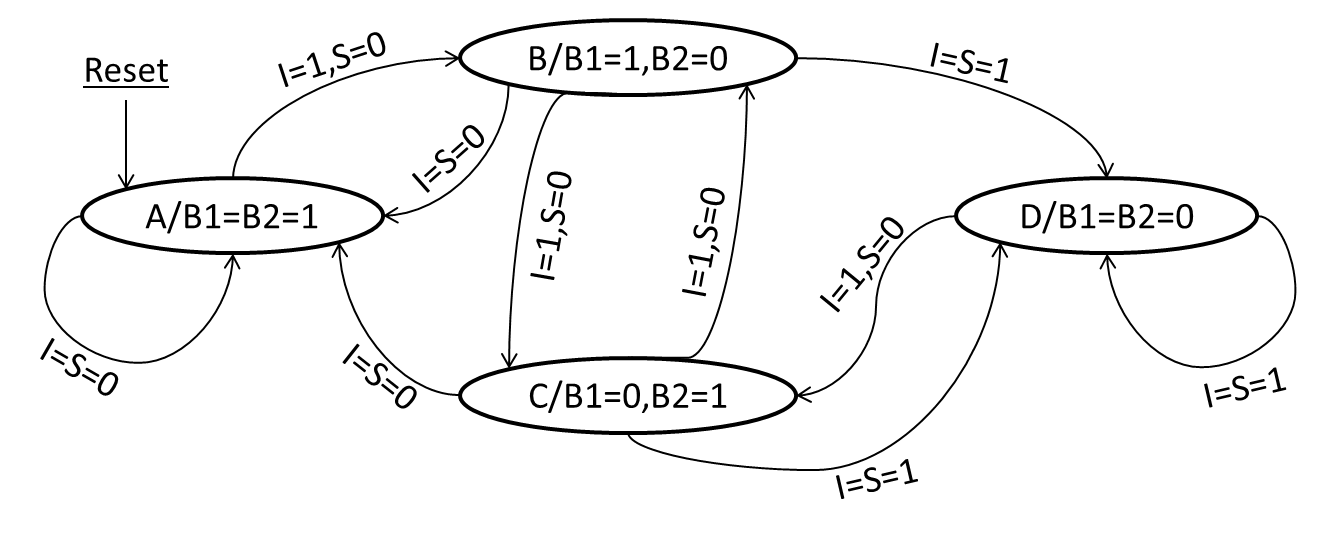
\includegraphics[scale=0.6]{../Ejercicio-1/moore1.png}
\end{center}
y la m\'aquina de estados de Mealy queda de la siguiente forma:
\begin{center}
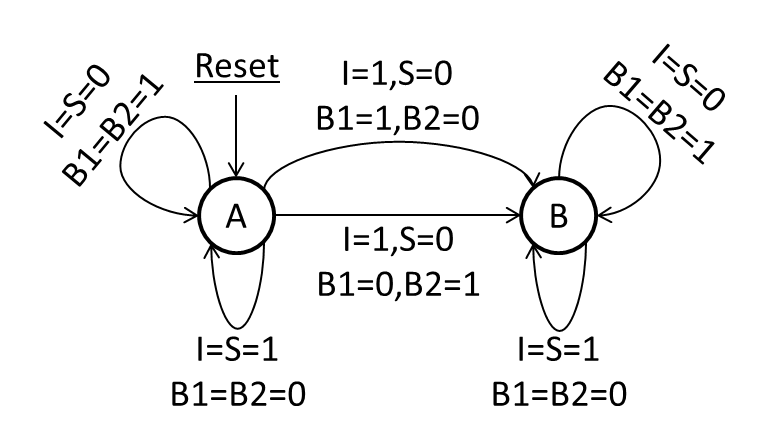
\includegraphics[scale=0.6]{../Ejercicio-1/mealy1.png}
\end{center}
Se puede ver que la mm\'aquina de estados de Mealy tiene menos estados que la de Moore ya que la salida depende de la entrada adem\'as del estado.

\subsection{Tabla de Estados}
A partir de los diagramas de estados, se procede a armar las tablas de estados de cada m\'aquina. Asignando a los estados como: A = 00, B = 01, C = 10 y D = 11, la tabla de estados de Moore queda de la siguiente forma:
\begin{center}
	\begin{table}[h!]
		\begin{center}
			\caption{Tabla de Estados de Moore}
  			\begin{tabular}{|c|c|c|c|c|}
			    \hline
			    \multirow{2}{*}{Present State} &
			    \multicolumn{3}{c|}{Next State} &
			    \multirow{2}{*}{Output} \\
			    \cline{2-4} & 
			    I=S=0 & I=1,S=0 & I=S=1 & \\
			    \hline
			    y2 y1 & Y2 Y1 & Y2 Y1 & Y2 Y1 & B2 B1 \\
			    \hline
			    0 0 & 0 0 & 0 1 & x x & 1 1 \\
			    \hline
			    0 1 & 0 0 & 1 0 & 1 1 & 0 1 \\
			    \hline
			    1 0 & 0 0 & 0 1 & 1 1 & 1 0 \\
			    \hline
			    1 1 & x x & 1 0 & 1 1 & 0 0 \\
			    \hline
			\end{tabular}
		\end{center}
	\end{table}
\end{center}
Y asignando a los estados como: A = 0 y B = 1, la tabla de estados de Mealy queda de la siguiente forma:
\begin{center}
	\begin{table}[h!]
		\begin{center}
			\caption{Tabla de Estados de Mealy}
  			\begin{tabular}{|c|c|c|c|c|c|c|}
			    \hline
			    \multirow{2}{*}{Present State} &
			    \multicolumn{3}{c|}{Next State} &
			    \multicolumn{3}{c|}{Output} \\
			    \cline{2-7} &
			    I=S=0 & I=1,S=0 & I=S=1 & I=S=0 & I=1,S=0 & I=S=1 \\
			    \hline
			    y & Y & Y & Y & B2 B1 & B2 B1 & B2 B1 \\
			    \hline
			    0 & 0 & 1 & 0 & 1 1 & 0 1 & 0 0 \\
			    \hline
			    1 & 1 & 0 & 1 & 1 1 & 1 0 & 0 0 \\
			   \hline
			\end{tabular}
		\end{center}
	\end{table}
\end{center}
\subsection{Mapas de Karnaugh}
A continuaci\'on se procede a obtener las ecuaciones l\'ogicas de cada tabla de estados.\\
Empezando con la tabla de estados de Moore, se obtiene:\\
Para Y1: \\
\begin{center}
	\begin{Karnaug}
	    \contingut{0,0,0,x,1,0,1,0,x,x,x,x,x,1,1,1}
	    \implicant{12}{10}{blue}
   		\implicantcostats{4}{14}{green}
	\end{Karnaug}
\end{center}
Donde se extrae que Y1 = S + y1*I.\\
Para Y2: \\
\begin{center}
	\begin{Karnaug}
		\contingut{0,0,0,x,0,1,0,1,x,x,x,x,x,1,1,1}
    	\implicant{12}{10}{blue}
	    \implicant{5}{15}{green}
	\end{Karnaug}
\end{center}
Donde se extrae que Y2 = S + $\overline{y1}$*I.
\\
Para B1: \\
\begin{center}
	\begin{Karnaughquatre}
		\contingut{1,1,0,0}
    	\implicant{0}{1}{blue}
	\end{Karnaughquatre}
\end{center}
Donde se extrae que B1 = $\overline{y2}$.
\\
Para B2: \\
\begin{center}
	\begin{Karnaughquatre}
		\contingut{1,0,1,0}
    	\implicant{0}{2}{blue}
	\end{Karnaughquatre}
\end{center}
Donde se extrae que B2 = $\overline{y1}$.\\
Y con estas ecuaciones ya es posible diseñar el circuito de Moore.
Ahora se obtendr\'an las ecuaciones l\'ogicas a partir de la tabla de estados de Mealy:

Para Y: \\
\begin{center}
	\begin{Karnaughvuito}
		\contingut{0,1,x,0,1,0,x,1}
    		\implicant{7}{6}{blue}
    		\implicant{1}{1}{red}
   		\implicantcostats{4}{6}{green}
	\end{Karnaughvuito}
\end{center}
Donde se extrae que Y = $\overline{S}$*I*$\overline{y}$ + y*(S + $\overline{I}$).
\\
Para B1: \\
\begin{center}
	\begin{Karnaughvuito}
		\contingut{1,1,x,0,1,0,x,0}
    		\implicant{0}{1}{blue}
   		\implicantcostats{0}{6}{green}
	\end{Karnaughvuito}
\end{center}
Donde se extrae que B1 = $\overline{y}$*$\overline{s}$ + $\overline{I}$.
\\
Para B2: \\
\begin{center}
	\begin{Karnaughvuito}
		\contingut{1,0,x,0,1,1,x,0}
    		\implicant{4}{5}{blue}
   		\implicantcostats{0}{6}{green}
	\end{Karnaughvuito}
\end{center}
Donde se extrae que B2 = y*$\overline{s}$ + $\overline{I}$.
Y con estas ecuaciones ya es posible diseñar el circuito de Mealy.

\section{Circuitos L\'ogicos y Simulaci\'on en GTKWave}
Como ya se tiene lo necesario para diseñar y simular los circuitos, se los diseña quedando de la siguiente forma:
Circuito utilizando la m\'aquina de estados de Moore:
\begin{center}
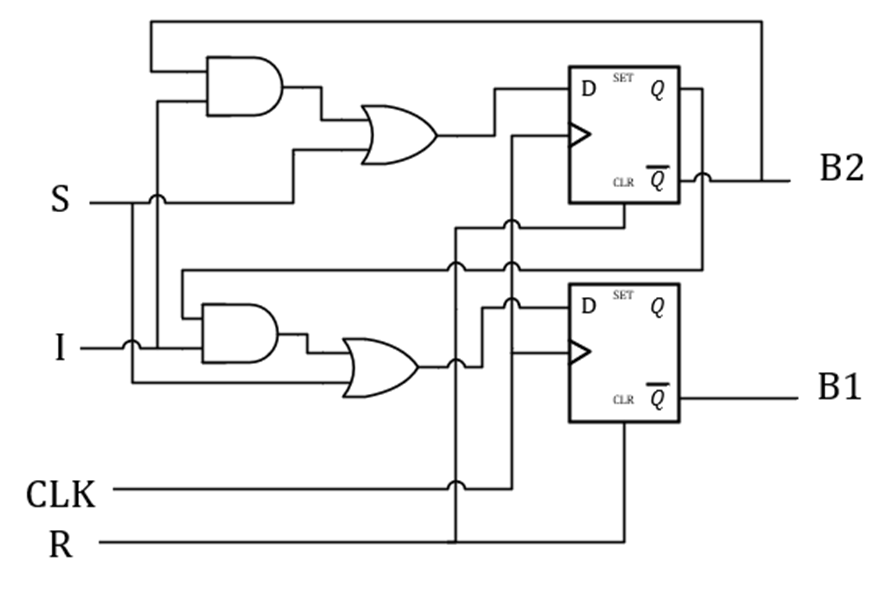
\includegraphics[scale=0.75]{../Ejercicio-1/moore3.png}
\end{center}
Al simular el circuito en GTKWave se obtiene lo siguiente:
\begin{center}
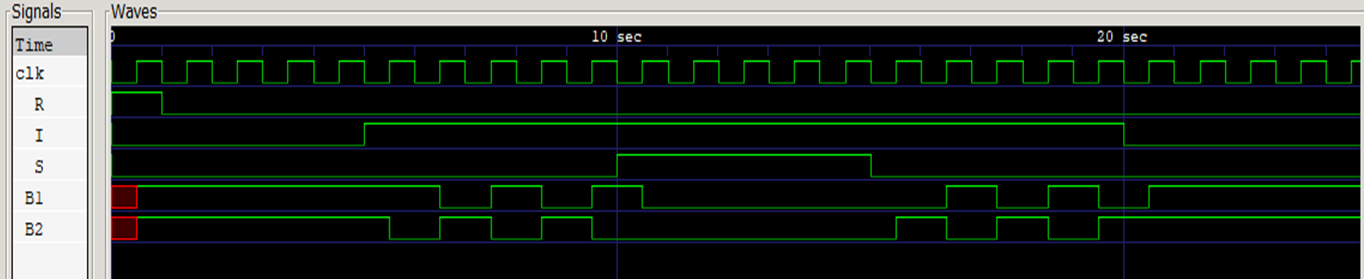
\includegraphics[scale=0.5]{../Ejercicio-1/moore2.png}
\end{center}
Circuito utilizando la m\'aquina de estados de Mealy:
\begin{center}
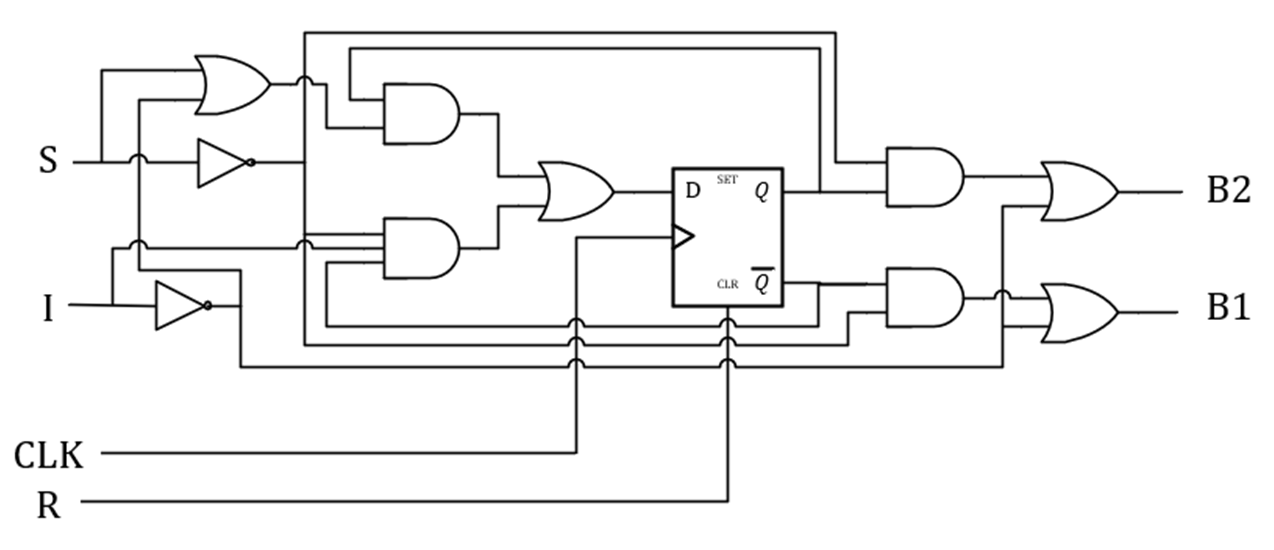
\includegraphics[scale=0.6]{../Ejercicio-1/mealy3.png}
\end{center}
Al simular el circuito en GTKWave se obtiene lo siguiente:
\begin{center}
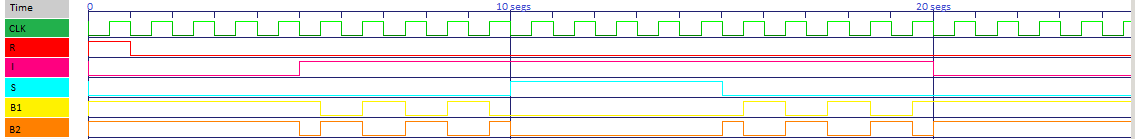
\includegraphics[scale=0.5]{../Ejercicio-1/mealy2.png}
\end{center}
La gran diferencia que se puede observar en la simulación es que la salidas est\'an desplasadas entre s\'i exactamente un ciclo de clock. Eso se debe a que el circuito el cual fue implimentado con Mealy responde m\'as r\'apido ya que su salida depende tanto de la entrada como del estado. En cambio el circuito el cual fue implementado con Moore solo depende del estado.